\documentclass{article}
\usepackage[utf8]{inputenc}

\title{IF677 -INFRA-ESTRUTURA DE SOFTWARE}
\author{Vinícius felipe Barbosa}
\date{Novembro 2019}

\usepackage{natbib}
\usepackage{graphicx}

\begin{document}

\maketitle

\section{Introdução}
Este curso faz parte da tríade hardware, software e comunicação, que é a base da construção de praticamente qualquer sistema de computação atual. O objetivo aqui é apresentar os conceitos e sistemas de software básicos de um computador, que compreende a introdução aos sistemas concorrentes e aos sistemas operacionais, sejam eles mono-computador ou distribuídos.
\citep{chamado1}
\begin{figure}[h!]
\centering
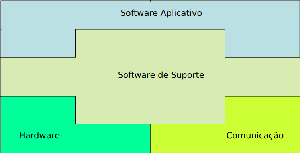
\includegraphics[scale=1.2]{img.jpg}
\citep{chamado2}
\caption{Relações}
\label{fig: img}
\end{figure}
\section{Relevância}
A disciplina de Infra-Estrutura de Software visa fazer com que os alunos entendam o funcionamento dos sistemas de software que fornecem uma infra-estrutura através da qual aplicativos (browsers Web, editores de texto, planilhas eletrônicas, jogos, etc.) podem interagir com o hardware. Ao final da disciplina, os alunos devem apresentar uma compreensão dos principais mecanismos necessários para se construir tal infra-estrutura, considerando os dois papéis que ela desempenha: de mecanismo de abstração para a plataforma de hardware subjacente e de gerenciador de recursos diversos como memória, capacidade de processamento e dispositivos de armazenamento e de entrada e saída. Nesta disciplina, o software de infra-estrutura está dividido em duas partes: 
\begin{itemize}
\item O sistema operacional.
\item Middleware.
 \end{itemize}
 Essa disciplina funciona em harmonia com as outras duas disciplinas de infra-estrutura, a de hardware e a de comunicação, e juntas as três fornecem um panorama razoavelmente completo sobre o funcionamento de um sistema computacional.
 \citep{chamado1}
 \section{Relações com outras disciplinas}
 A disciplina de Infra-Estrutura de Software se relaciona com as disciplinas:
 \begin{itemize}
 \item Infra-Estrutura de Hardware
 \item Infra-Etrutura de Comunicação.
 \end{itemize}
 \citep{chamado3}
\bibliographystyle{plain}
\bibliography{vfb2}
\end{document}
